\chapter{Methodology}

This chapter describes the detailed methodology adopted for the design and implementation of the Quantum Retrieval-Augmented Generation (QRAG) framework. The methodology focuses on integrating classical Retrieval-Augmented Generation (RAG) pipelines with Quantum Natural Language Processing (QNLP) techniques to address syntactic ambiguity in user queries. The system is designed as a hybrid architecture that selectively applies quantum processing for complex linguistic structures while maintaining efficiency for simpler queries.

\section{System Architecture Overview}

The QRAG system follows a modular and decoupled architecture consisting of multiple layers, including query processing, ambiguity detection, hybrid execution, retrieval, and response generation. Each component operates independently while communicating through well-defined interfaces, ensuring scalability and maintainability.

The overall workflow begins with user input, followed by structural analysis of the query. Based on the detected complexity, the system routes the query to either a classical or quantum processing pipeline.

\section{Model Pipeline Steps}

The complete processing pipeline of the QRAG system is summarized in Table~\ref{tab:pipeline_steps}, which outlines the sequence of operations performed from query input to response generation.

\begin{table}[htbp]
    \centering
    \caption{QRAG Model Pipeline Steps}
    \label{tab:pipeline_steps}
    \begin{tabular}{|c|p{4cm}|p{7cm}|}
        \hline
        \textbf{Step} & \textbf{Component} & \textbf{Description} \\
        \hline
        1 & User Input & User submits natural language query \\
        \hline
        2 & Preprocessing & Tokenization, normalization, and POS tagging \\
        \hline
        3 & Ambiguity Detection & Detects syntactic ambiguity using predefined signatures \\
        \hline
        4 & Routing Mechanism & Routes query to classical or quantum pipeline \\
        \hline
        5 & Classical Pipeline & SpaCy parsing and vector-based retrieval for simple queries \\
        \hline
        6 & Quantum Pipeline & VQC-based encoding and entanglement for ambiguous queries \\
        \hline
        7 & Contextual Realignment & Selects correct interpretation of the query \\
        \hline
        8 & Retrieval Module & Fetches relevant documents from vector database \\
        \hline
        9 & Generation Module & LLM generates final response \\
        \hline
    \end{tabular}
\end{table}

The execution and visualization of these pipeline steps are illustrated in Figure~\ref{fig:pipeline_steps_viz}.

\begin{figure}[htbp]
    \centering
    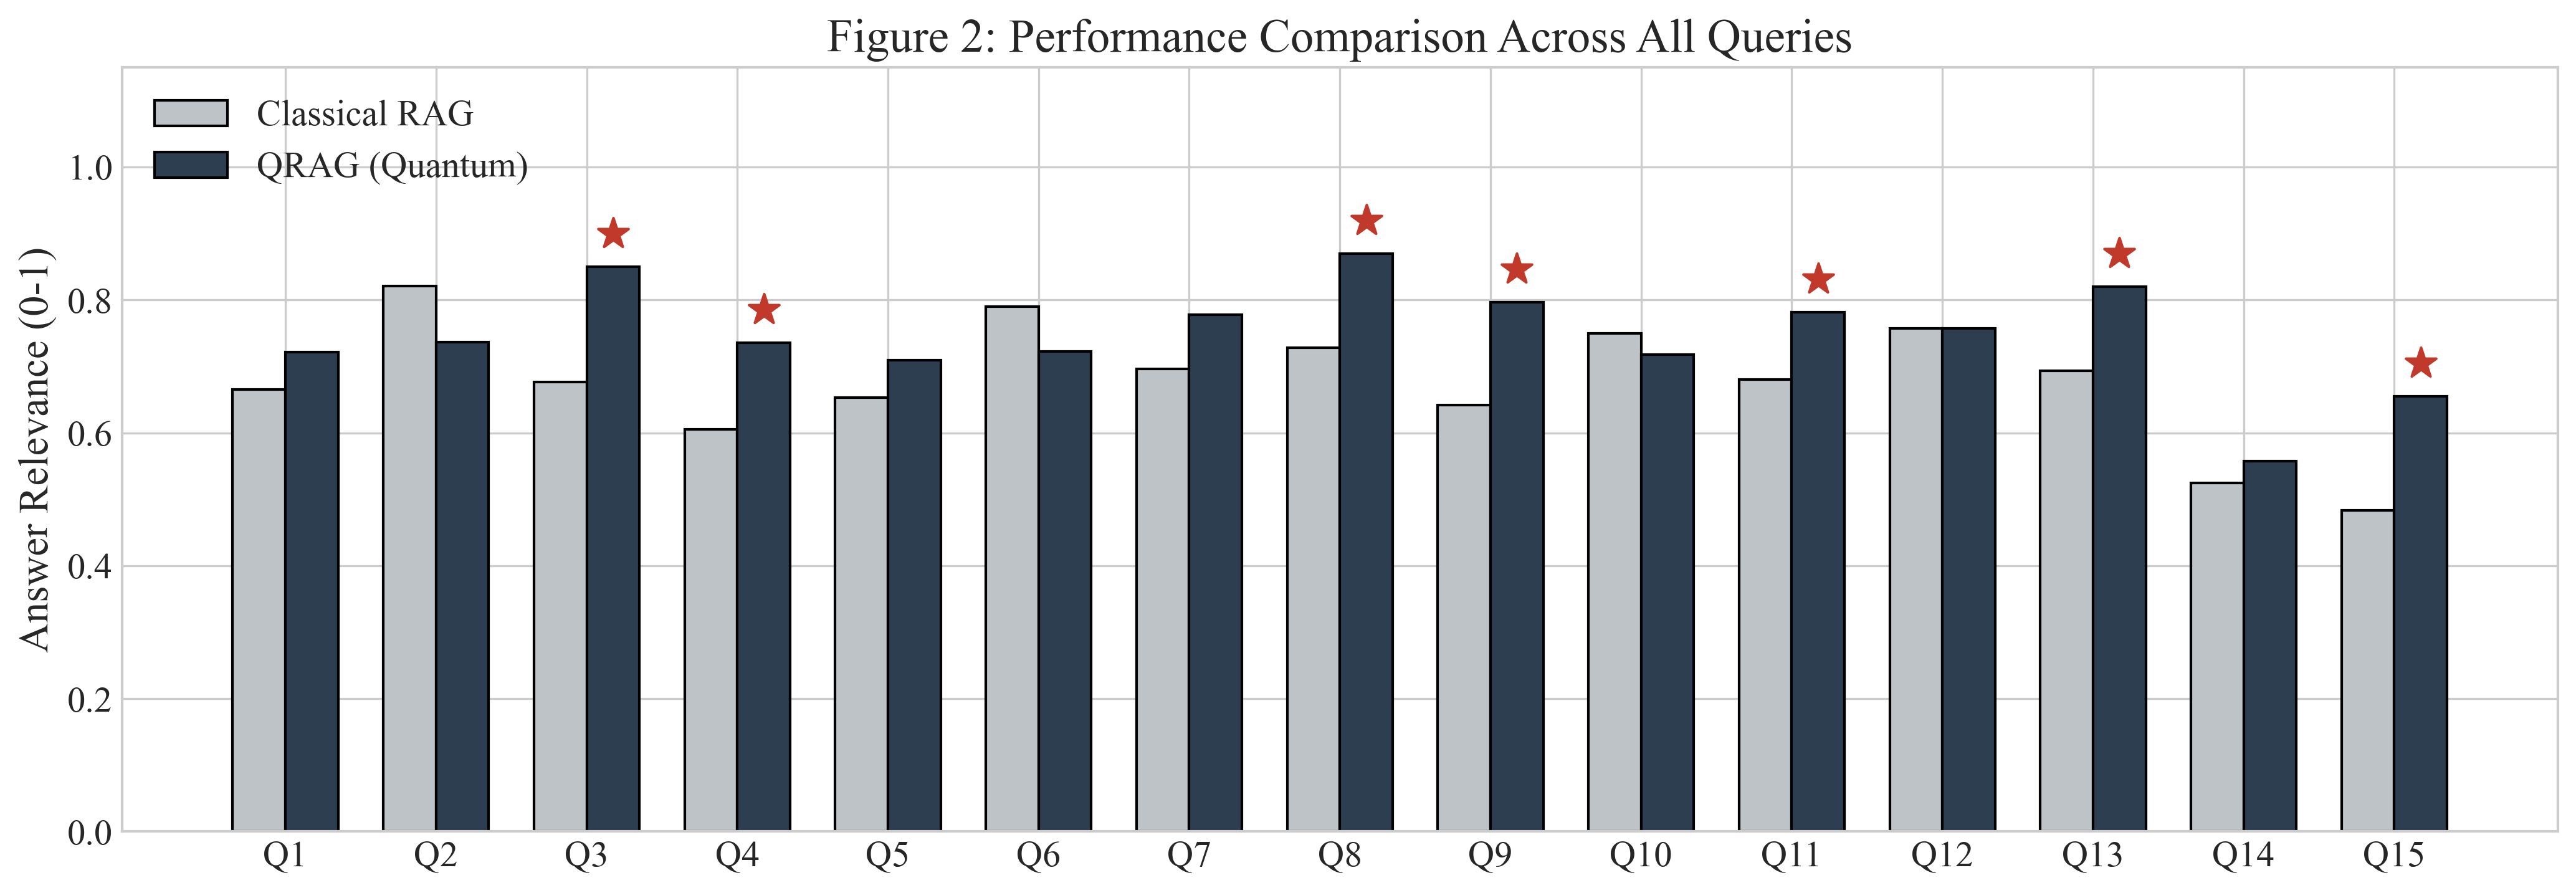
\includegraphics[width=0.45\textwidth]{assets/Journal/figure2.png}
    \hfill
    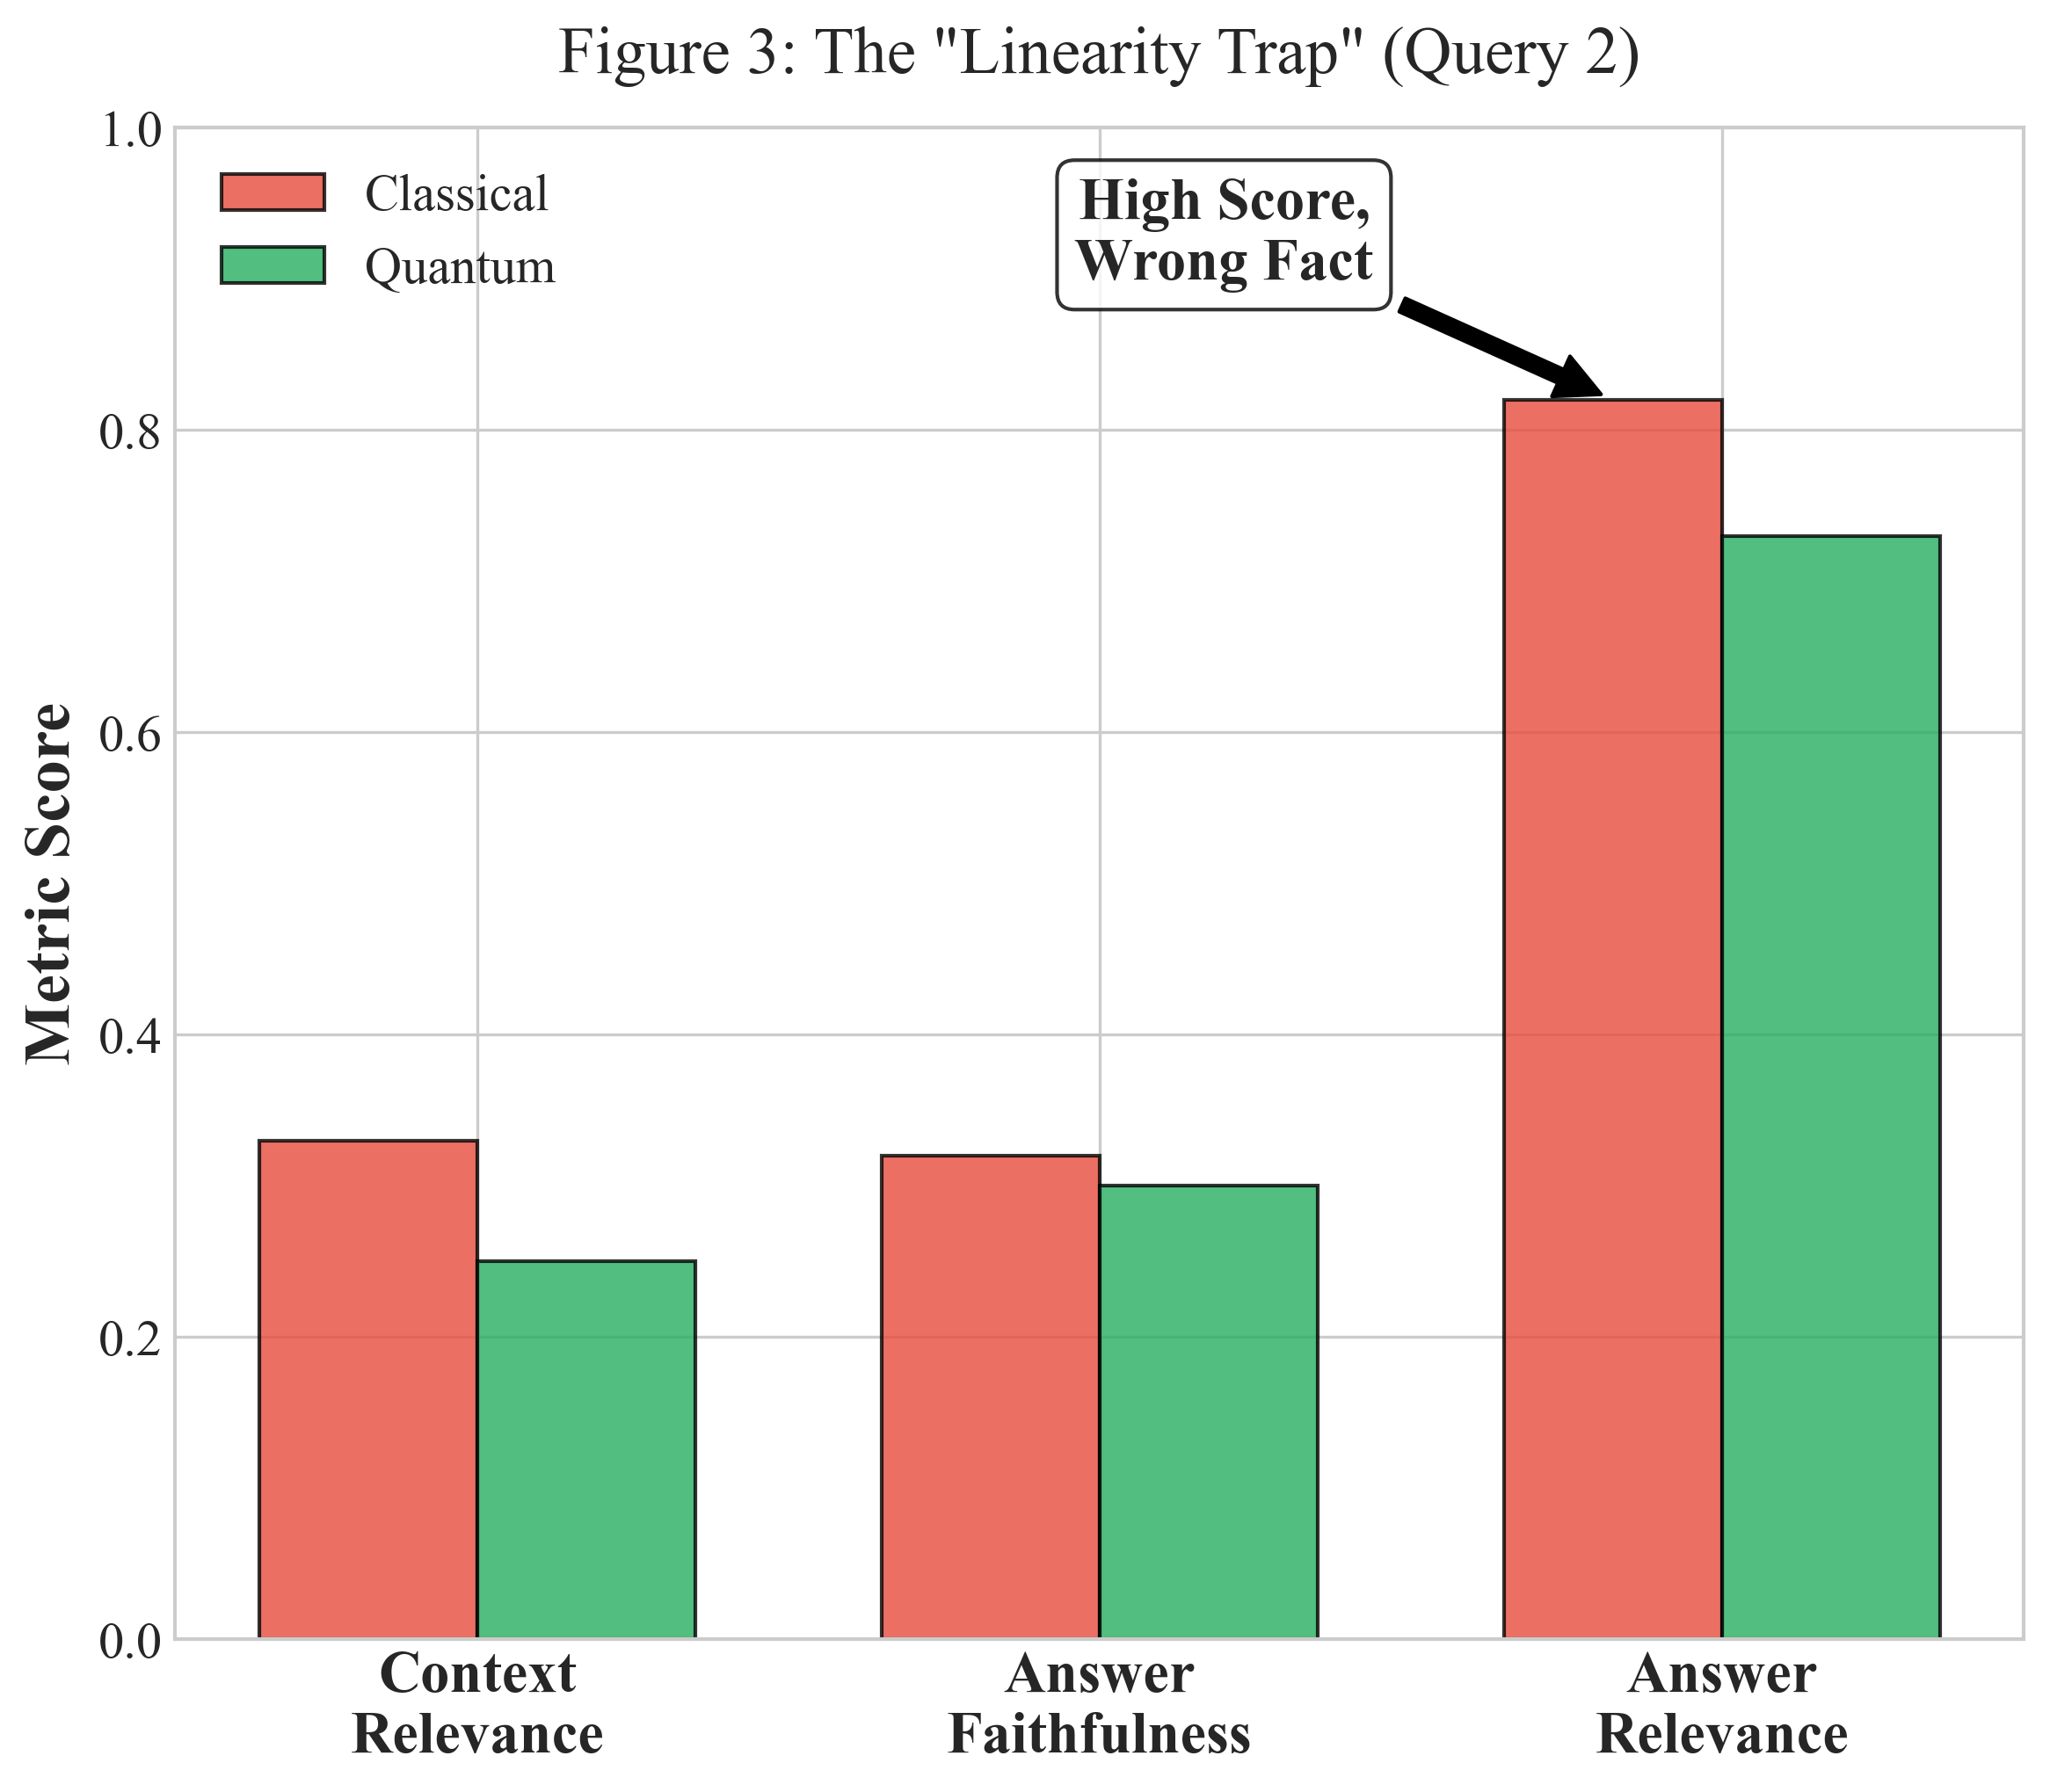
\includegraphics[width=0.45\textwidth]{assets/Journal/figure3.png}
    \\
    \vspace{0.5cm}
    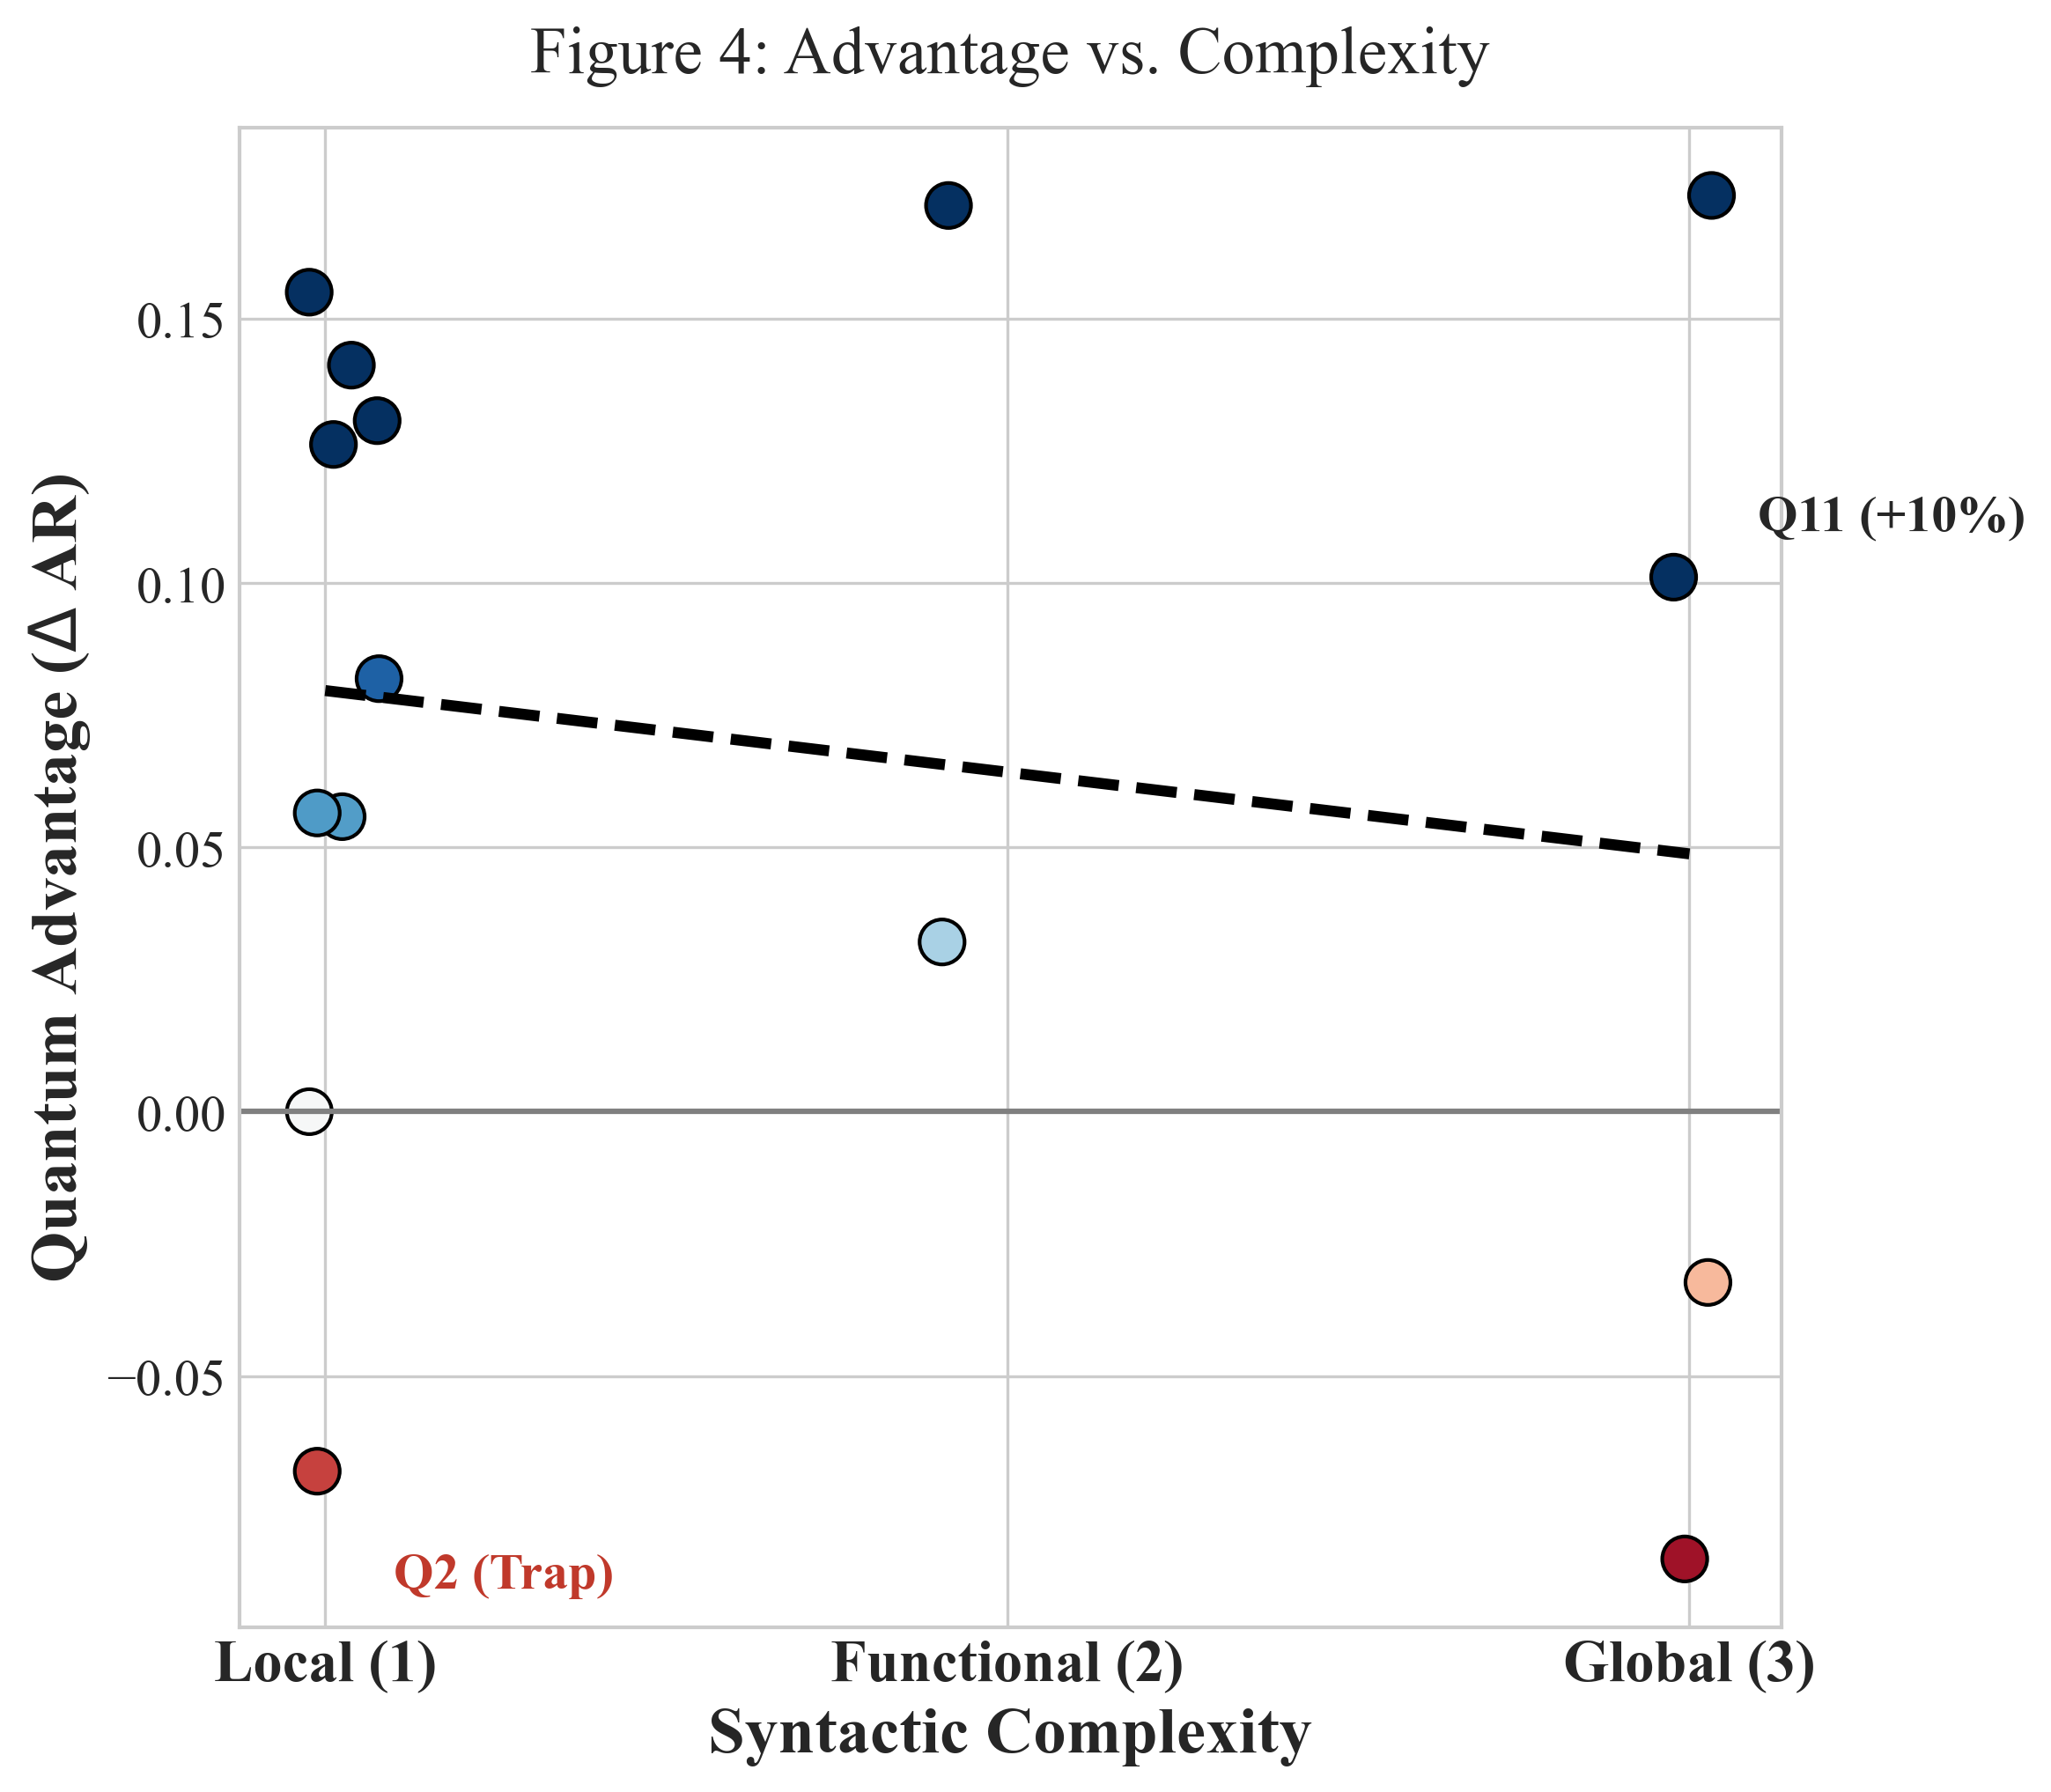
\includegraphics[width=0.5\textwidth]{assets/Journal/figure4.png}
    \caption{Visualization of QRAG model pipeline execution steps.}
    \label{fig:pipeline_steps_viz}
\end{figure}

\section{Data Preparation and Corpus Construction}

The system utilizes a heterogeneous dataset comprising approximately 30,000 records stored in MongoDB. The dataset is preprocessed using normalization, tokenization, and embedding generation to enable efficient vector-based retrieval.

\section{Ambiguity Detection Strategy}

A lightweight POS tagging mechanism is used to detect syntactic ambiguity. The system identifies patterns such as prepositional phrase attachment, reduced relative clauses, and coordination ambiguity. Queries matching these patterns are routed to the quantum pipeline.

\section{Algorithm Comparison}

A comparative analysis of classical and quantum approaches used in the system is presented in Table~\ref{tab:algorithm_comparison}. This comparison highlights the advantages of hybrid processing.

\begin{table}[htbp]
    \centering
    \caption{Comparison of Classical and Quantum Algorithms}
    \label{tab:algorithm_comparison}
    \begin{tabular}{|p{3cm}|p{4cm}|p{4cm}|p{3cm}|}
        \hline
        \textbf{Aspect} & \textbf{Classical Approach} & \textbf{Quantum Approach} & \textbf{Observation} \\
        \hline
        Model Type & SpaCy Parser / SGD & Variational Quantum Classifier (VQC) & Hybrid usage improves efficiency \\
        \hline
        Complexity Handling & Linear relationships & Non-linear relationships via Hilbert space & Quantum better for ambiguity \\
        \hline
        Processing Speed & Fast & Slower & Classical preferred for simple queries \\
        \hline
        Accuracy (Ambiguous Queries) & Lower & Higher & Quantum shows advantage \\
        \hline
        Resource Requirement & Low & High & Selective usage required \\
        \hline
    \end{tabular}
\end{table}

\section{Classical Processing Pipeline}

The classical pipeline handles low-complexity queries using dependency parsing and vector-based retrieval. It ensures low latency and efficient processing for real-time applications.

\section{Quantum Processing Pipeline}

The quantum pipeline encodes queries into quantum states using rotation gates and models dependencies using entanglement (CZ gates). The circuit is executed on a quantum backend to determine the correct interpretation.

\section{Variational Quantum Circuit Design}

The Variational Quantum Circuit (VQC) consists of alternating rotation and entanglement layers, optimized using classical optimizers such as COBYLA. This enables the system to learn complex linguistic structures.

\section{Contextual Realignment}

The system refines query interpretation before retrieval, ensuring alignment between query intent and retrieved context. This significantly improves semantic accuracy compared to traditional RAG systems.

\section{Retrieval and Generation}

The disambiguated query is used to retrieve relevant documents from MongoDB Atlas. The retrieved context is passed to an LLM for generating the final response.

The structure of relationships between retrieved entities is illustrated in Figure~\ref{fig:retrieval_graphs}.

\begin{figure}[htbp]
    \centering
    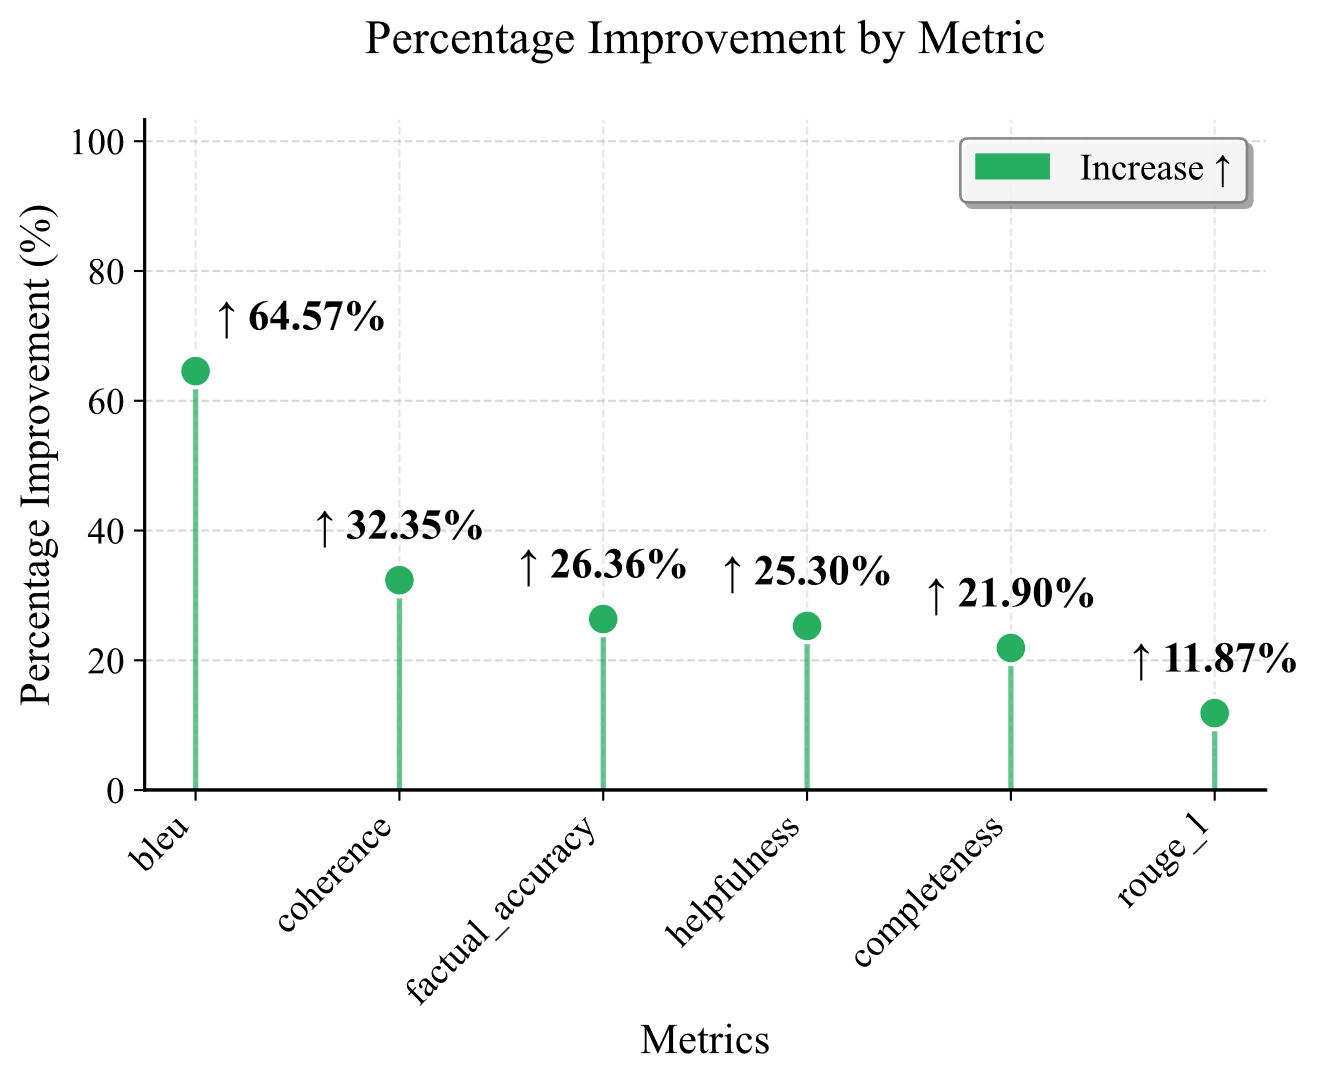
\includegraphics[width=0.48\textwidth]{assets/cicn/graph.png}
%    \hfill
%    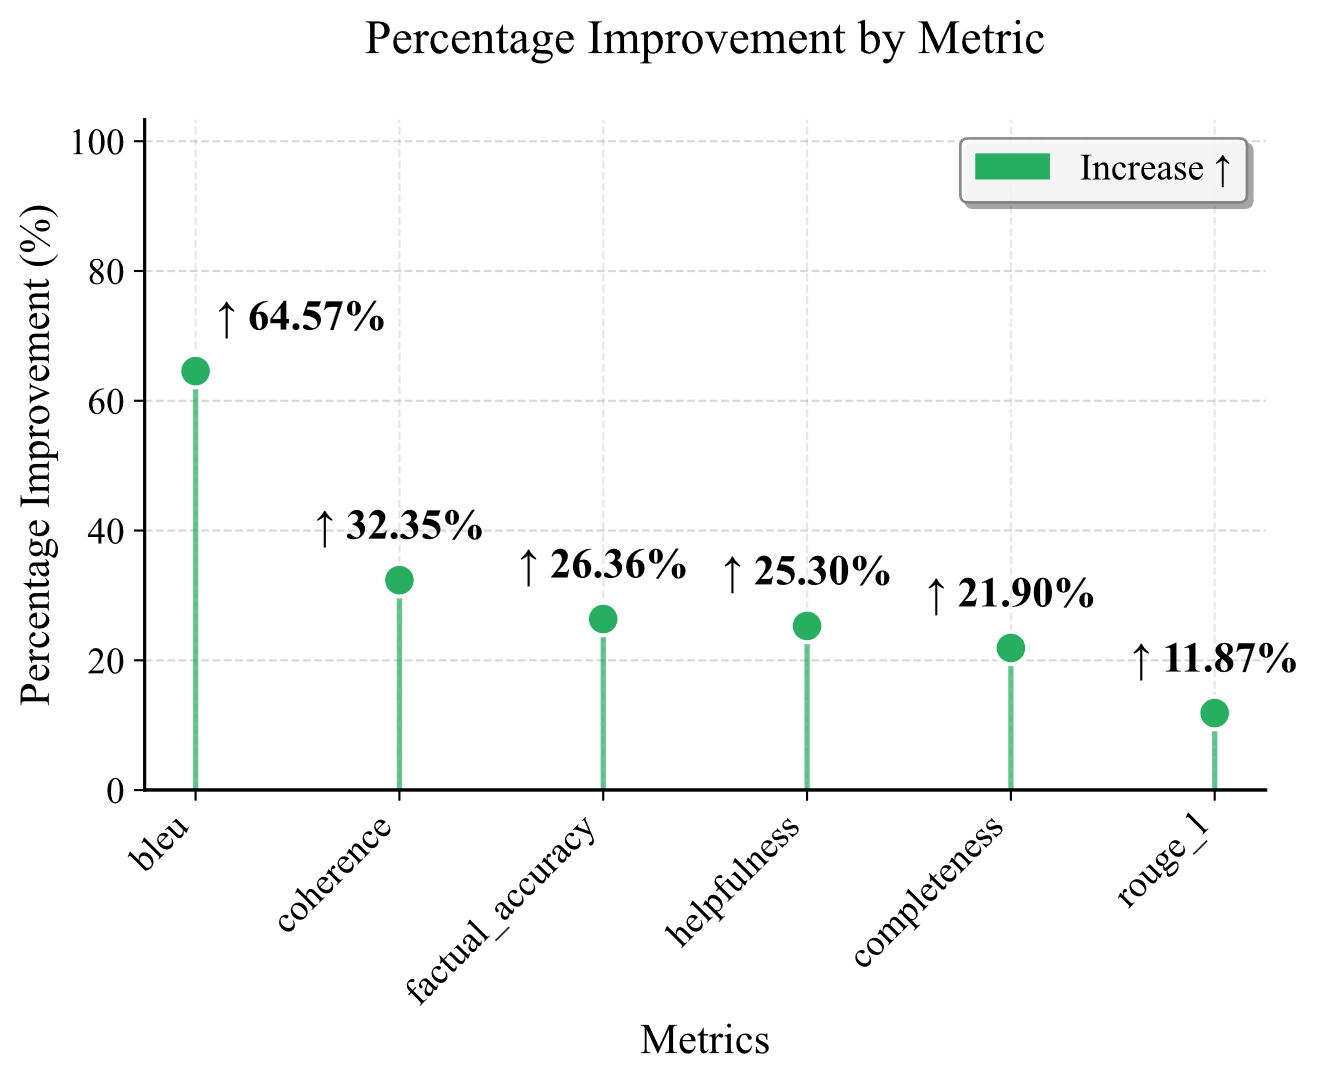
\includegraphics[width=0.48\textwidth]{assets/cicn/graph.png}
    \caption{Knowledge graph representations illustrating relationships between retrieved entities.}
    \label{fig:retrieval_graphs}
\end{figure}

\section{Evaluation Methodology}

The system is evaluated using an ambiguity-focused dataset. The evaluation metrics include:
\begin{itemize}
    \item Context Relevance (CR)
    \item Answer Faithfulness (AF)
    \item Answer Relevance (AR)
\end{itemize}

\section{Implementation Strategy}

The system is implemented using FastAPI (backend), React (frontend), MongoDB Atlas (vector storage), Neo4j (graph representation), and Qiskit (quantum execution), following a scalable cloud-native architecture.

\bigskip\noindent
The methodology combines classical efficiency with selective quantum processing to improve ambiguity resolution while maintaining performance and scalability.